\documentclass{article}
\usepackage[utf8]{inputenc}
\usepackage[colorlinks=true, allcolors=blue]{hyperref}
\usepackage{graphicx}
\usepackage{setspace}
\usepackage{parskip}

\title{Visual Analytics for Big Data (WMCS16000)\\
\large{Assignment 1}}
\author{Shaniya Hassan Ali (s3555496)
\\Carlos Huerta (s3743071) }
\date{22 September 2018}

\begin{document}

\maketitle

\doublespacing

%--- STEP 1 ---%
\section{Choose an Application Domain and Visualization Solution}

The visualization we have selected for this assignment is the \textbf{Rolling Stone's Top 500 Albums}. The visualization is available to view on tableau's public gallery. The link is given below
\\
\\
\url{https://public.tableau.com/en-us/s/gallery/rolling-stones-top-500-albums?gallery=votd} 
\\
\\
"The 500 Greatest Albums of All Time" is a 2003 special issue of American magazine Rolling Stone, and a related book published in 2005 \cite{rstone-wiki}. The lists presented were compiled based on votes from selected rock musicians, critics, and industry figures, and predominantly feature American and British music from the 1960s and the 1970s.

In 2012, Rolling Stone published a revised edition of the list drawing on the original and a later survey of albums in the 2000s. It was made available in "bookazine" format on newsstands in the US from April 27 to July 25. The new list contained 38 albums not present in the previous one, 16 of them released after 2003 \cite{rstone-wiki}.

While its not very visually complex as it is very easily understandable by any layman and fairly easy to use, it does contain high dimensional data. The visualization shows the band/groups with 5 or more albums in the top 500, the decade with the most albums in the top 500 and the primary genre with most albums in the top 500. It is interactive wherein more specific album/artist details can be extracted and viewed for closer inspection in the top 500. The visualization also deals with different types of data such as time series in terms of the years from 1954-2011, categorical data such as the genre, hierarchical data which in this case could be the genre as well. It approaches visualization with high dimensional data about the music industry, specifically how genre, age of release and artist can affect how an album is ranked higher or lower by experts of the industry.

We will use this visualization and compare it against another visualization that represents the music timeline \cite{music-timeline} and possibly use it to improve the Rolling Stone's Top 500 visualization. We will overview the common questions they address, how a certain information is portrayed differently and what additional information is required to make the current visualization more effective.

Our main challenge is to critically analyze the current visualization and create better improved ones that is easily understood by the general audience as well as answer key problems that the visualization is trying to solve or the high and low level information that is been conveyed.
    
Below we see a typical snapshot of the Rolling Stone's Top 500 visualization:

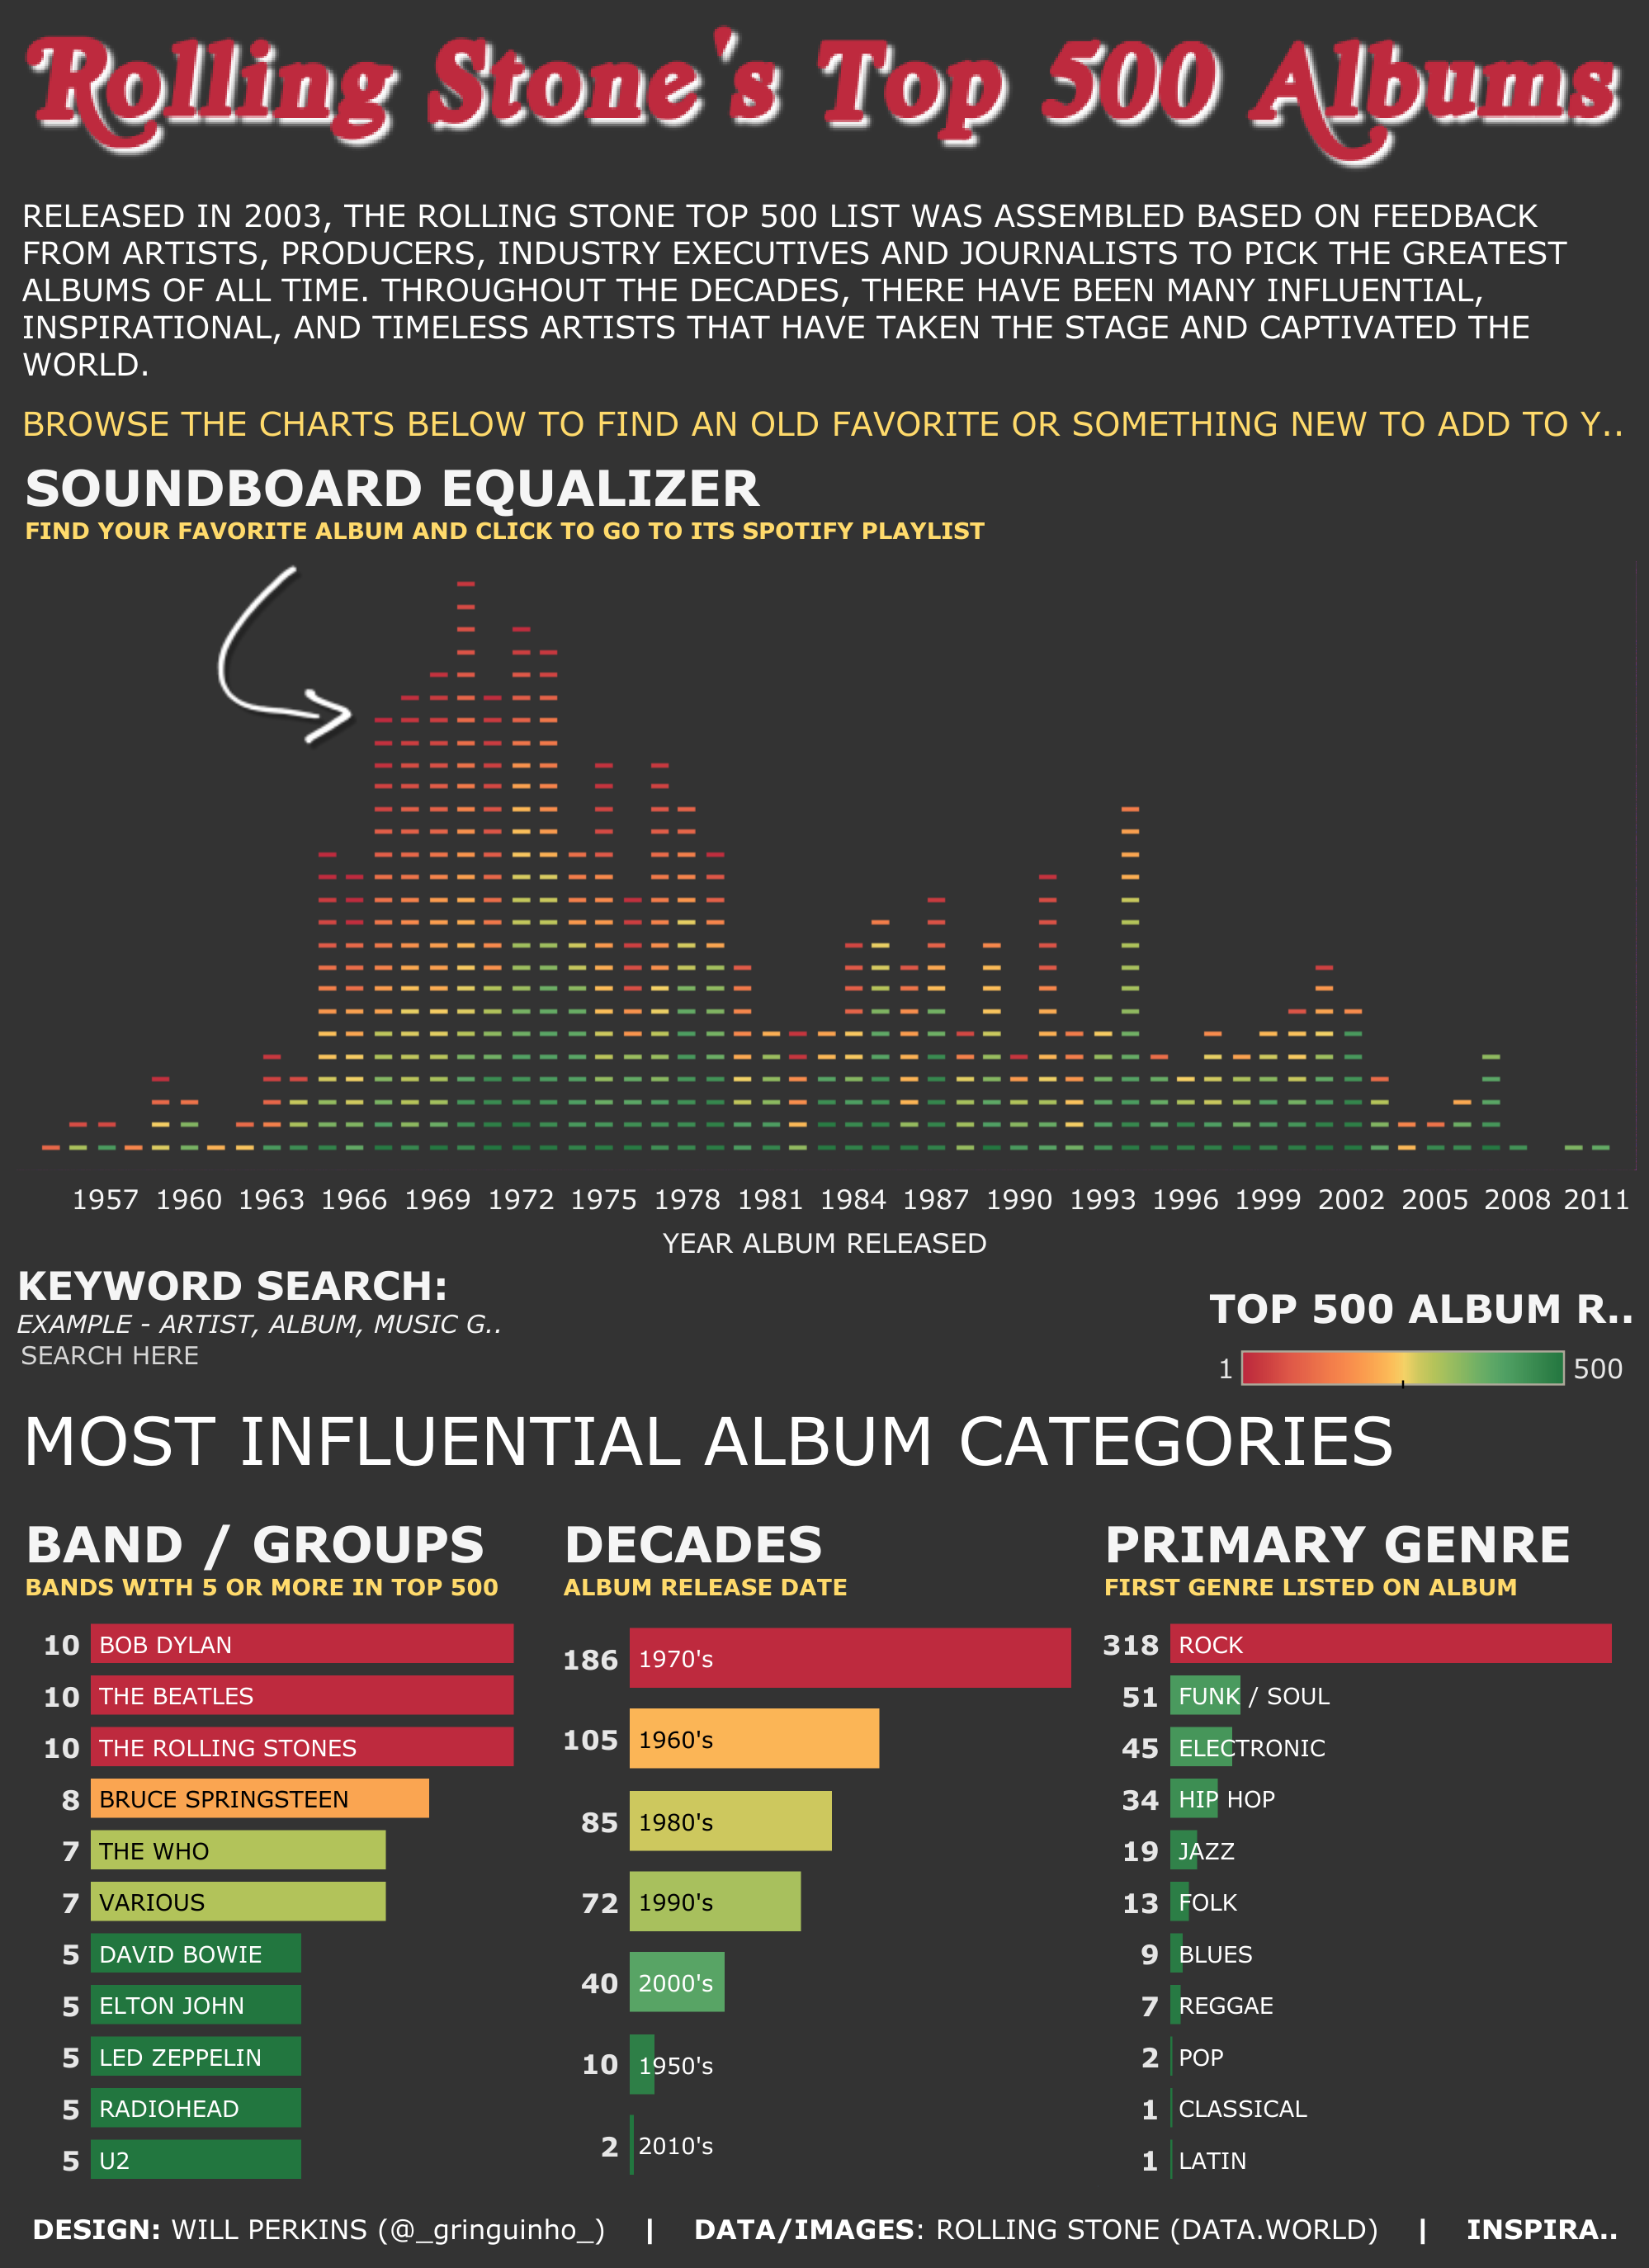
\includegraphics[width=\textwidth]{VisualAnalytics/Assignment1/images/rolling-stone-main.png}

Below we have also provided the snapshot of the music timeline

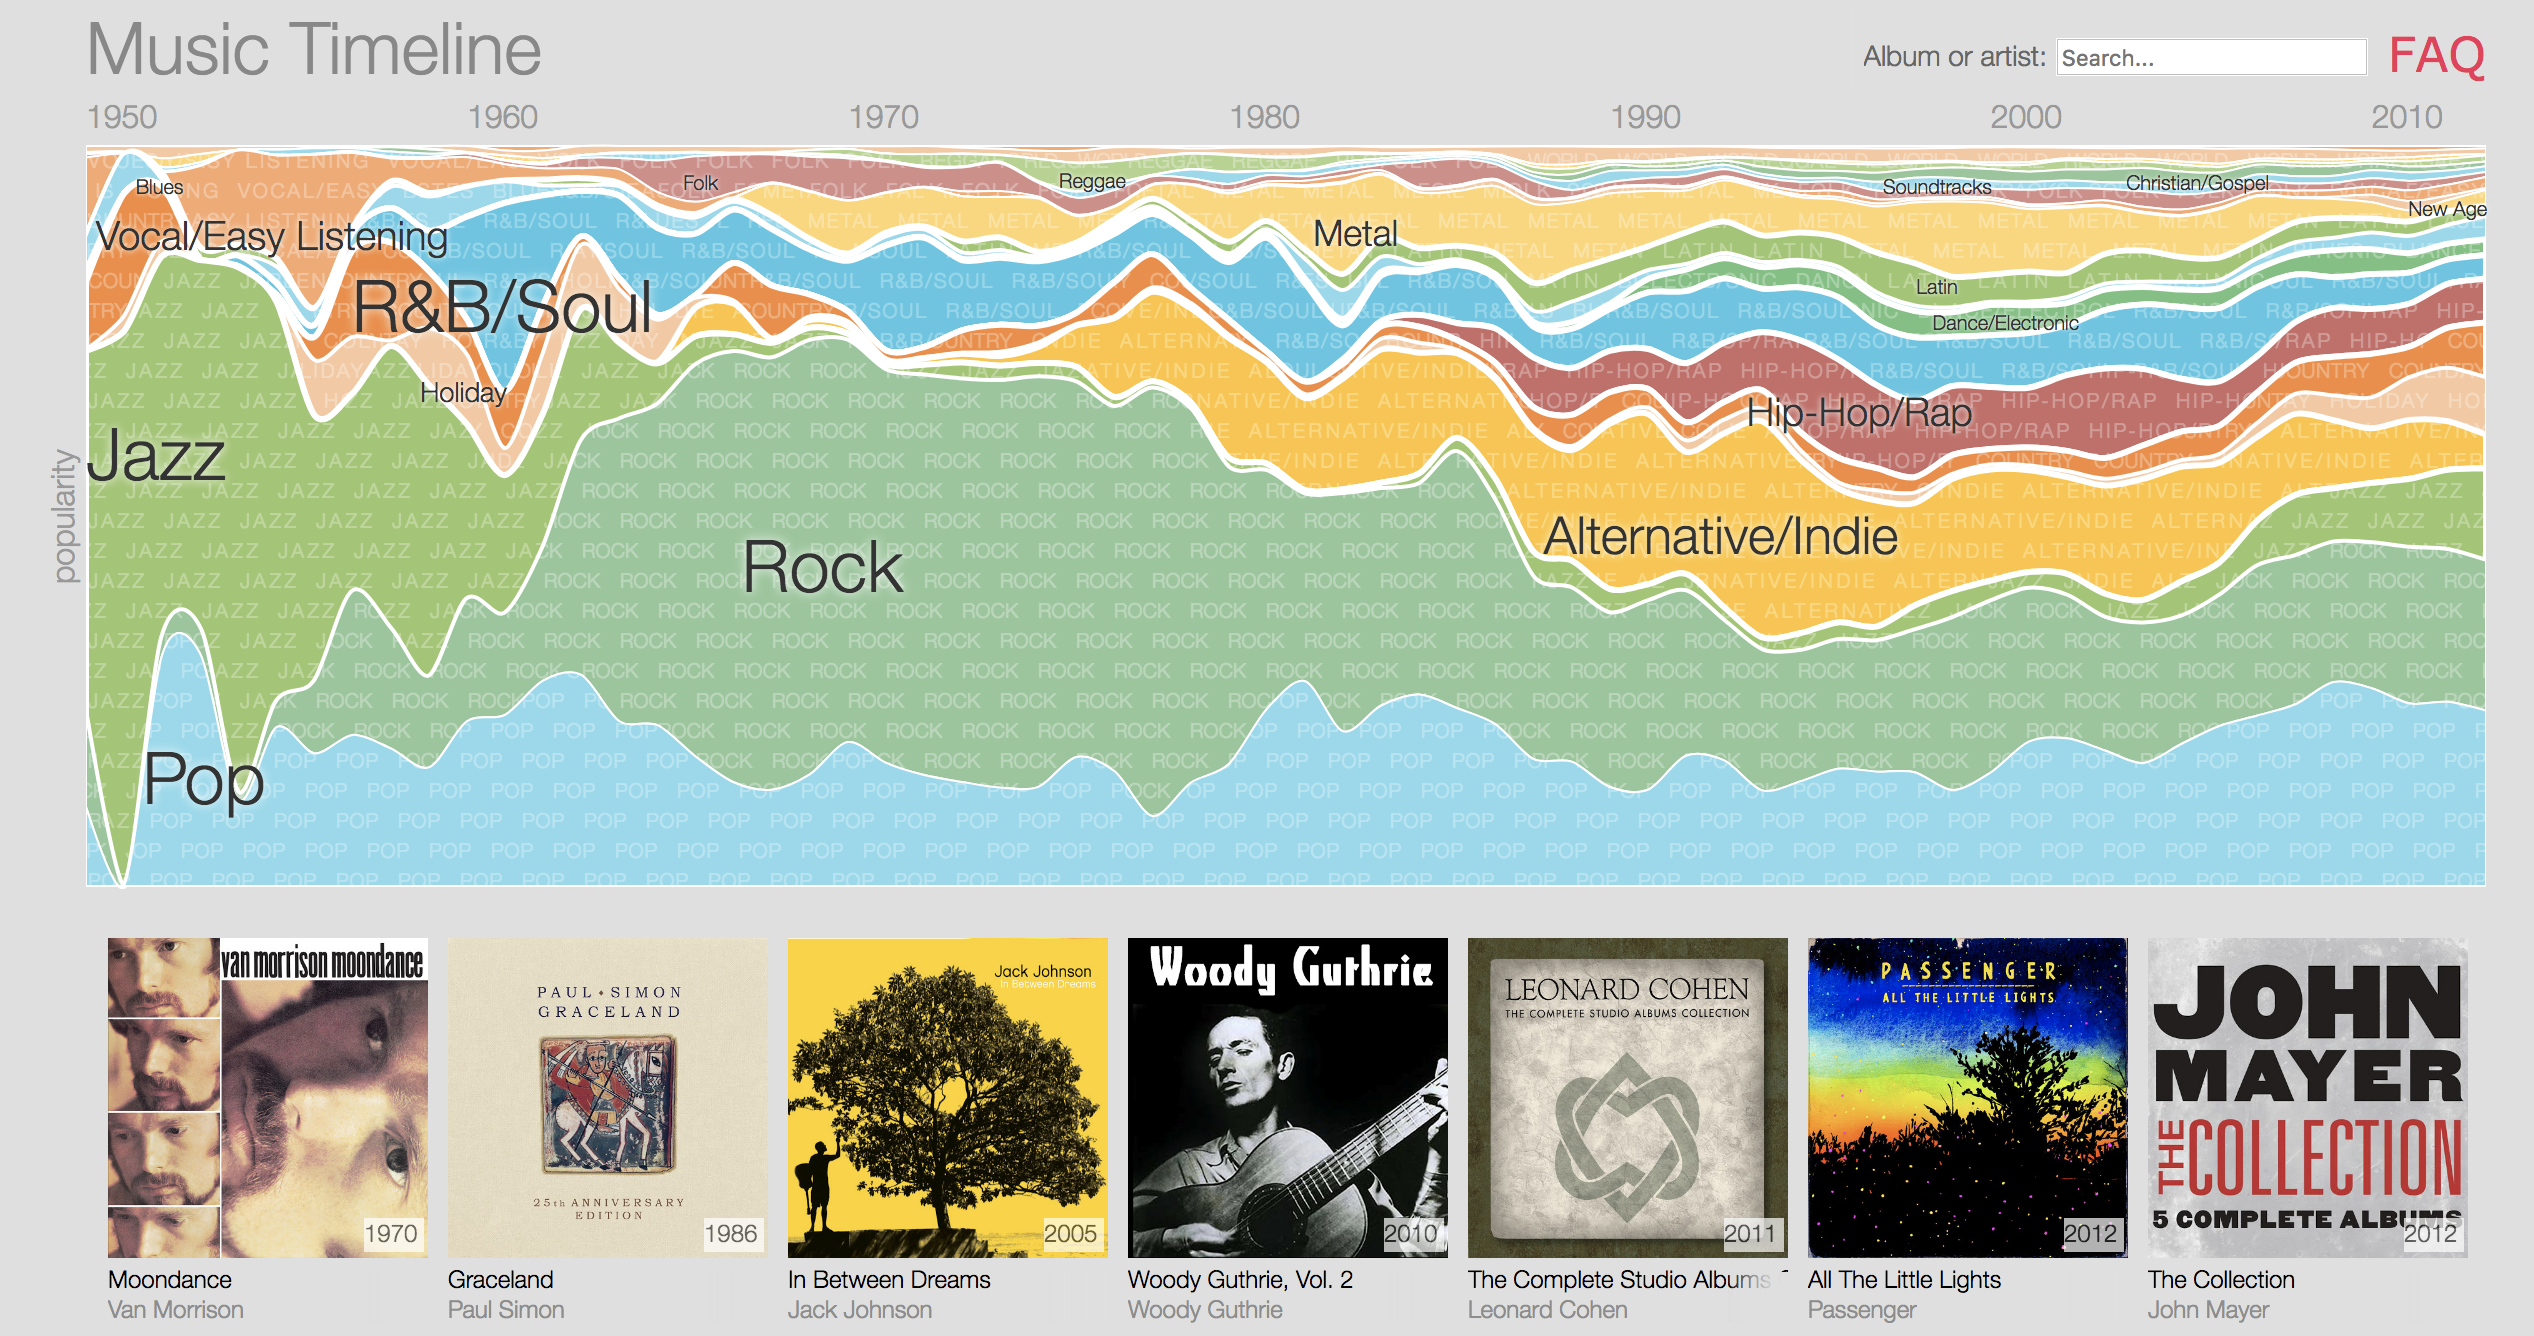
\includegraphics[width=\textwidth]{VisualAnalytics/Assignment1/images/music-timeline.png}

%--- STEP 2 ---%
\section{Description of the underlying problem}

\subsection{What questions does this visualization aims to answer?}

In its premise, the visualization is quite easily understood and the problem it is trying to solve is pretty simple. What are the top 500 albums spanning the decades from 1960s to early 21st century? However, on closer inspection, we can find many links between the data that is represented. These relations give rise to even more complex and high level understanding of the music evolution and the artists that contributed to it. 

\textbf{Concrete Questions}
\begin{itemize} 
    \item What is the best album of all time?
    \item What is the best genre of music?
    \item Which year or decade has been the least successful in terms of musical quality? 
    \item Which year or decade has been the most successful in terms of musical quality? 
    \item Which artist band or group has the most highly rated albums?
\end{itemize}

\textbf{Higher level Questions}
\begin{itemize} 
    \item How can we compare individual genres in terms of quality against one or the other?
    \item Which artist band or group is or was the best?
    \item Is there an overall decay in the quality of music during the last few years or is just our nostalgia and perception?
\end{itemize}

\textbf{Summary}
\begin{itemize} 
    \item How can we create a map of how music rating (quality) has evolved over time in terms of genre, band and decade?
\end{itemize}

These are not easy questions to answer specially for a subject like music in which perception and personal preference plays a huge role on determining the answer to these questions. Maybe we are all biased towards a certain genre of music? 

\subsection{Users}
This type of visualization which are rooted from the entertainment/music domain are mainly used by music enthusiasts, artists, record labels as well as the general public. It re-establishes the top artists throughout the decades while also highlighting any new artists that has made the list. Users are also given the interactivity to select an album and listen to it on Spotify which is a nice touch on the visualization.

% In this case any music fanatic can benefit from the visualization as well as music industry experts and artists trying to get famous. The most common user the "music lover" will benefit by knowing in the opinion of the industry experts which bands they could listen to. Maybe application consumers or producers off music streaming apps such as spotify users will appreciate music suggestions other than their recommended list.
        
% The music retailer, store or cafe can chose which too add to their inventories, or playlists "good music" in order to attract more clients and sell their products more easily. This raises the question, Does "good music" is equivalent to popular music?

\subsection{Purpose}

The Rolling Stone magazine's top 500 albums spanning decades is compiled based on the votes from rock musicians, critics and industry figures. While it gives a good overview of the top albums, it is based on a small niche of the overall population and not the ultimate list for top 500 albums. Experts in the industry could use this visualization against a more complete voting system to find relationships and links between these visualizations.

It also represents which genre has better or worse reception as well as which decade has the most albums with high ratings. All of these information will give a much closer look at the evolution of music as well as what is considered as good quality music.

% The main purpose of the visualization is to determine a visual and quick way to represent quality of music albums and their evolution across the last century in terms of analysis like the best or worst genre of music and in terms of presentation how has music quality evolved over time.

%--- STEP 3 ---%
\section{Data Description}
\subsection{Characterization of our data}

Our data is multidimensional each single record of our data contains: Genre, Artist, Year of Release, Band/Group, Sub-genre and Ranking.

\textbf{Types and value ranges of our data}
\begin{itemize} 
    \item \textbf{Genre} Data attribute discrete, qualitative, categorical. This data field describes what musical genre does a certain album belongs to. It ranges from the categorical types of: Rock, Funk/Soul, Electronic, Hip-Hop, Jazz, Folk, Blues, Reggae, Pop, Classical and Latin.
    \item \textbf{Artist} Data attribute discrete, qualitative, categorical, this data field describes which Artist was the author of a concrete album, this data varies a lot we have artists like David Bowie, Elthon John, Bob Dylan and many more, it is a countable set but with many dimensions.
    \item \textbf{Year of Release} Data attribute discrete, quantitative, interval. This field indicates at what year was a certain album released, it ranges from 1955 to 2011.
    \item \textbf{Band/Group} Data attribute discrete, qualitative, categorical. This field indicates which Band or was responsible for recording an specific album, this data field has certain similarities with "Artist" but can vary, because a certain album can have a single Artist, but it was recorded by a certain Group, this field ranges from "The Doors", "The Beatles" etc.
    \item \textbf{Sub-genre} Data attribute discrete, qualitative, ordinal. This data field depends entirely on Genre, each Genre has specific types of Sub-Genres, for example: Rock can have, alternative rock and hard rock as sub-categories. This field can be used to describe a relation of belongingness or subset in terms of Genre.
    \item \textbf{Rank} Data attribute discrete, quantitative, interval. This field is the hearth of our visualization everything will revolve around ranking, Ranking ranges from $1$ to $500$, on a side-note we must not confuse the natural ordering of numbers and on this case the $1$ album is greater in terms of ranking than the $500$ album. 
    
\end{itemize}

\section{Visual Design Study}
In this section, we will look at how the 
\subsection{Type of Visualization}
\subsection{Visual Encoding}
\subsection{Improvements}

\section{Description of Findings}

\bibliographystyle{unsrt}
\bibliography{bibliography}
    
\end{document}